% Define document class
\documentclass[twocolumn]{aastex631}

\newcommand{\flatiron}{\affiliation{Center for Computational Astrophysics, Flatiron Institute, New York, NY 10010, USA}}
\newcommand{\stonybrook}{\affiliation{Department of Physics and Astronomy, Stony Brook University, Stony Brook NY 11794, USA}}
\usepackage{amsmath}
\usepackage{amssymb}
\usepackage{bm}
\usepackage{xcolor}
\definecolor{rb4}{HTML}{27408B}
\newcommand{\kw}[1]{{\color{rb4}[KW: #1 ]}}
\newcommand{\wf}[1]{\textcolor{cyan}{WF: #1}}
\newcommand{\kb}[1]{\textcolor{pink}{#1}}
% \setlength{\floatsep}{0cm}
% \setlength{\textfloatsep}{0cm}
% \setlength{\belowcaptionskip}{-5pt}
% \setlength{\abovecaptionskip}{-5pt}
% Begin!
\begin{document}
\title{Backpropagating Gravitational wave events}

\pacs{}

\author{Kaze W. K. Wong} 
\email{kwong@flatironinstitute.org}
\flatiron

\author{Katelyn Breivik}
\flatiron

\author{Will M. Farr}
\email{will.farr@stonybrook.edu}
\flatiron
\stonybrook


\date{\today}

\begin{abstract}
One promising way to extract information about stellar astrophysics from
gravitational wave catalogs is to compare the catalog to the outputs of
population synthesis modeling with varying physical assumptions.  The parameter
space of physical assumptions in population synthesis is high-dimensional and
the choice of parameters that best represents the evolution of a binary system
may depend in an as-yet-to-be-determined way on the system's properties; indeed,
measuring the variation of population synthesis parameter settings with binary
properties is one of the principal ways to extract information about binary
astrophysics from catalogs. Here we propose an inference pipeline to
simultaneously infer stellar progenitor parameters (e.g. zero-age main sequence
masses) and population synthesis parameter settings controlling modeled binary
evolution from individual gravitational wave observations of merging compact
binaries.  Our pipeline can efficiently explore the high-dimensional space of
population synthesis settings and progenitor system properties for each system
in a catalog of gravitational wave observations.  We apply our pipeline to
observations in the third LIGO Virgo Kagra Gravitational Wave Transient Catalog
(GWTC3).  We showcase the effectiveness of this pipeline with a detailed study
of the progenitor properties and population synthesis settings that produce
mergers like the observed GW150914.
\end{abstract}

%\maketitle

\section{Introduction}
As the detection rate of gravitation waves (GWs) from merging
double-compact-object (DCO) binaries increases with the sensitivity of the
ground-based GW detector network
\citep{Abbott2018,LIGOScientificCollaboration2015,Buikema2020,Tse2019,Acernese2015,Acernese2019,Aso2013,Akutsu2021},
we are beginning to constrain the astrophysical processes which shape the
evolution of GW progenitor populations. One of the most common ways to study
progenitor populations of GW mergers is through population synthesis simulations
for a host of formation environments including isolated binary stars, triple
systems, globular clusters, nuclear star clusters, AGN disks, and more
\citep{Mandel2022}. \wf{Moar citations here} Traditionally in these studies, the
population is studied through a Monte-Carlo approach.  Using theoretically
motivated distributions of initial parameters (age, metallicity, masses, orbital
separations, eccentricities, etc), initial populations are evolved with fixed
astrophysical assumptions (population synthesis parameter settings)to produce a
synthetic catalog of mergers which can be compared of observations from
ground-based GW detectors.



%As the rate of detection of gravitational-wave (GW) increases with the sensitivity of the \kb{ground-based} GW detector network \kw{cite},
%understanding astrophysical processes related to progenitors of GW events through analyzing a population of GW events has become more popular \kw{cite}. 
%\kb{I think we can reword the end of this previous sentence -- I should come back to it.}
%A very common way to study the origin of detected GW events is through population synthesis simulations \kw{cite} \kb{cite Mandel \& Broekgaarden review},
%which evolve populations of various kinds of binaries to form populations of GW events. \kb{Do we want to do isolated only here? or other channels?}
%\kb{The process to forward model a population of GW events relies on random samples }
%Forward modelling of a population of GW events start with sampling a set of initial binary parameters from some distributions related to the progenitor population,
%such as the initial mass function or star-formation history,
%then evolve each individual members according to the physics of interest until some stopping criteria is met.
%This usually mean either a merger event or the binary system stays stable for a Hubble time.
%After this, one can collect all the GW emitting binaries in the synthetic population and compare to the observed population.

While forward modelling entire populations has been the canonical pathway to
compare simulations and GW observations, it is not necessarily the most
efficient way to constrain the underlying physical processes, represented by
population synthesis ``hyperparameters,'' which drive the evolution of the
population.  \wf{I would not turn to ``skepticism'' here; instead, I would say
something like [but worded better] ``it is likely that the hyperparameter
settings that best represent the evolutionary physics vary across progenitor
parameter space in unknown ways, which makes the modeling very expensive if you
want to produce an entire population with one hyperparameter setting.
Additionally, comparing at the level of populations is not as efficient as
comparing event-by-event.  Ideally, we would like to \emph{hierarchically}
combine several observations to directly constrain the progenitor population
\emph{and} hyperparameter settings all at once from the observed catalog.''  I
see that these points come in the next paragraph, so one thing you could do is
dramatically shorten this paragraph and use it to lead into the next one.} One
of the most common skepticism of population synthesis studies is that these
studies employ simulation sets which often cover a small subdomain of the entire
parameter space of uncertain physics, or only vary one uncertain process per
simulation (e.g. common envelope efficiency) while holding all others fixed to
some "default" values. On top of this, these values are often not calibrated to
data. Even with recent developments in using emulators to speed up the
simulation process, training the emulators still requires a significant amount
of computation to cover a wide range of uncertainty. As an example, to emulate a
model with $10$ parameters, the simplest way to construct a training set of
simulations is to run a grid which varies combinations of uncertain physics. For
10 uncertain physical processes, if we consider $2$ variations for each physical
process this would still require $1024$ simulations. Because population
synthesis simulations require hundreds to thousands of cpu hours, training an
emulator which spans a high dimensional uncertainty space remains an
impossibility at present.

\kw{Reorganizing discussion related to Jeff's work such that it doesn't seem like our method is just an extension of DartBoard.}

This compounds with the fact that there is no guarantee the entire population
should share the same fixed hyperparameters, as is often assumed in most
population synthesis studies. This suggests that there could be a large
(possibly infinite) family of hyper-parameter distributions required to compare
data to simulations which span the full set of uncertain physical models.
However, this issue is not a fundamental issue, but an apparent obstacle which
arises from an inefficient approach to the problem. Furthermore, each binary
system could in principle come from a different formation environment and hence
have different progenitor parameters as well as hyperparameters, which define
uncertain physics associated with each environment. In this case, it is
advantageous to determine the posterior density in the progenitor and
hyper-parameter joint space for each individual binary system, then perform
population in analyses in that space. \citet{Andrews2021} (hereafter A21) used
\texttt{DartBoard} \citep{Andrews2018} to determine the ZAMS parameters which
produce GW150914-like BBH merger based on posterior samples for GW150914 and a
fixed set of hyperparameters which define assumptions for how isolated
binary-star interactions proceed using \texttt{COSMIC}, a binary population
synthesis code \citep{Breivik2020}. Crucially, the method did not vary the
hyperparameters while sampling the posterior density of the ZAMS parameters,
which limit its capability to be applied to understand a population of binary
systems.  \wf{This sounds sort of aggressive against DartBoard, and we probably
don't want to do that.  Instead, maybe re-focus the 'graph on
\emph{distinguishing} our method from DB; less DB sux and more ``here is how we
are not DB.''}

In this paper, we propose a method to "backward" model each GW event to its
progenitor state while allowing the hyperparameters to vary across their full
range of physical uncertainty following a two-stage process. First, we solve a
root finding problem to obtain guesses that are likely to produce the desired
system properties in the joint progenitor--hyper-parameter space. We then sample
the posterior in the joint space with Markov chain Monte Carlo (MCMC) algorithm
that is initialized using the roots found in the previous stage; the
initialization step makes the burnin and convergence of the MCMC stage
considerably faster than initializing with random parameter choices
\citep{Andrews2018,Andrews2021}. The rest of the paper is structured as follows:
We detail our method in Sec. ~\ref{sec:method}. In Sec. ~\ref{sec:result}, we
show the results of applying our method to a number of real events. We discuss
the implications of this work and future direction in Sec.
~\ref{sec:discussion}.

\section{Method}
\label{sec:method}

We define the parameters that describe the progenitor's zero age main sequence (ZAMS) properties
masses and eccentricity as progenitor parameters $\bm{\theta'}$, the parameters
that control different uncertain physical prescriptions such as wind strength and common
envelope efficiency as hyperparameters $\bm{\lambda}$, and random variables
that affect certain stochastic process such as whether CO natal kick unbinds a
binary as $\bm{X}$. To avoid clutter in the following derivation, we denote all
the parameters related to mapping a particular progenitor system into a GW event
collectively as evolutionary parameters $\bm{\Theta}$, which includes
$\bm{\theta'}$, $\bm{\lambda}$, and $\bm{X}$.

Once all the parameters including a particular draw of all the random variables
represented by $\bm{X}$ are known, the population synthesis code is a
deterministic function that transforms the properties of the progenitors into
the GW parameters $\bm{\theta}$:
\begin{equation}
    \bm{\theta} = \bm{f}\left( \bm{\Theta} \right).
\end{equation}
The mapping $\bm{f}$ from $\bm{\Theta}$ to $\bm{\theta}$ can be many-to-one
due to degeneracies in the different physical processes and initial parameters  
of the GW event progenitors.
In order to draw inferences about $\bm{\Theta}$ from GW data, we
must be able to evaluate the likelihood of that data at fixed progenitor
parameters, namely
\begin{equation}
    p\left( d \mid \bm{\Theta} \right) = p\left( d \mid \bm{\theta} = \bm{f}\left( \bm{\Theta} \right) \right).
\end{equation}
The equality holds because the likelihood depends only on the gravitational waveform generated by
parameters $\bm{\theta}$ to which the progenitor parameters map onto.  In principle
this likelihood could be computed at arbitrary values of $\bm{\Theta}$ using the
same machinery that is used to estimate source parameters in GW
catalogs \citep{Veitch2015,Ashton2019,Romero-Shaw2020,GWTC-3} to develop samples
of progenitor parameters, hyperparameters, and random variables in
$\bm{\Theta}$ from a posterior density.

Since the GW likelihood function
ultimately depends only on the GW parameters $\theta$, and GWTC3 already has samples over these parameters from a posterior density 
\begin{equation}
    p\left( \bm{\theta} \mid d \right) \propto p\left( d \mid \bm{\theta} \right) \pi_\mathrm{GW} \left( \bm{\theta} \right),
\end{equation}
where $\pi_\mathrm{GW}$ is the prior density used for sampling,
we can save the computation cost associated with evaluating the GW likelihood by rewriting the posterior 
density of $\Theta$ in terms of the posterior density of $\theta$, namely

\begin{align}
    p(\Theta | d) = \frac{p(\theta(\Theta)| d) \pi(\Theta)}{\pi_\mathrm{GW}(\theta(\Theta))},
\end{align}
which we apply a kernel density estimator to the posterior samples released in GWTC3 to estimate $p(\theta(\Theta)|d)$.

Including hyperparameters and random variables %in the sampling 
drastically increases the dimensionality of the problem,
which makes the sampling process more computationally expensive to converge.
To speed up the convergence, we first solve a root-finding problem to find points that are close to the bulk of the posterior density of a GW event,
then we use those points to initialize a set of chains in the MCMC process.

%The root-finding procedure is described as follows:
For each posterior sample point in the GW-observable space,
we can find the corresponding evolutionary parameters by solving an optimization problem that minimizes 
the mean square difference between the GW event parameters and evolutionary parameters as:

\begin{align}
\mathcal{L}(\bm{\Theta},\bm{\theta}) = ||f(\bm{\Theta})-\bm{\theta}||^2.
\label{eq:loss}
\end{align}

In principle, we should only accept solutions that exactly reproduce the LVK posterior samples in the GW-observable space.
However, it is not feasible to achieve such a condition in practice, therefore we relax the condition in eq.~\ref{eq:loss} 
to a small acceptance threshold. For this study, we picked a threshold of $10^{-2}$. To make sure we find a reasonably 
complete set of progenitor parameters that corresponds to the posterior sample point, we use 1000 different initial guesses 
in solving the optimization problem. As long as the solution fulfills the acceptance criteria, the root is as valid as all 
other roots that fulfill the same acceptance criteria, \emph{regardless to its initial guess}.
This means, we have the freedom to choose the set of initial guesses however we think might benefit the optimization.

Most of the points in the evolutionary parameter space do not produce DCO mergers in a Hubble time. For systems that do not merge, 
we set the binary masses to be $0$ such that the gradient for the same systems is also $0$ and leads the root finder to get stuck on 
its first step.{\footnote{On a plateau of constant loss, the root finder performs no better than a random guess. 
Because of this, a root finder in a high dimensional space will require a significant amount of computation
to get close to a solution.}} Therefore, it is beneficial to choose initial guesses in region of the evolutionary parameter 
space that are likely to produce DCO mergers. To construct a list of initial guesses, we evolve a set of 
ZAMS parameters uniformly sampled from the initial binary parameter space, then keep the systems that 
merge within a Hubble time.

Retaining explicit control over random variables allows us to marginalize over their contribution, 
and thus allows us to focus on progenitor parameters and hyperparameters.
However, in practice most population synthesis codes (including \texttt{COSMIC} which we use in this study) 
define their random variables implicitly such that the random variables are drawn within the program instead of 
being passed as arguments. This means the function we use to evolve the binary is not fully deterministic.
Thus, even if the root-finding algorithm performs perfectly, forward modelling a set of roots does not 
guarantee that the simulated population reproduces exactly the set of posterior samples due to 
randomness in the evolution of each binary. To assure that the recovered progenitor and hyperparameters 
robustly correspond to the posterior in the GW-observable space, we forward model (or "reproject") the recovered 
evolutionary parameters to the GW-observable space to check whether the reprojected posterior agrees 
with the posterior given by the LVK collaboration. We use KL divergence to measure the agreement between the two posterior 
distributions as:
\begin{align}
D_{KL}(P||Q) = \int P(\bm{x}) \log(P(\bm{x})/Q(\bm{x})) dx.
\label{eq:KLdivergence}
\end{align}


A small KL divergence means the reprojected \texttt{COSMIC} posterior is similar to the original posterior in the 
observable space, and is thus a viable channel for that specific event. Otherwise, it either means \texttt{COSMIC} 
can only explain part of the posterior or cannot explain the event at all. This is completely expected behavior since 
\texttt{COSMIC}, and isolated binary evolution more generally, carries its own assumptions and is expected to 
fail in reproducing a subset of the event in GWTC3. One example of this are GW events with at least one component 
with mass above the pair instability supernova mass limit \kb{cite Farmer, and others}.
The reprojection could also be subject to stochasticity in the evolution of each binary
To account for this, we reproject the posterior multiple times with different random seeds and 
check whether the KL divergence varies significantly. A varying KL divergence means a particular GW event is subject 
to randomness in the evolution of the progenitor, and extra caution should be used when interpreting the result.


\section{Result}
\label{sec:result}
    
\begin{table*}[hbt!]
    \begin{center}
    \begin{tabular}{ l l l }
    \hline
    \hline
    Parameters &  Description & Optimization range\\
    \hline
    \hline
    Observables &\ &\  \\
    \hline
    \hline
    $m_{\rm 1, GW}$ & Primary mass of the GW event & NA \\
    $m_{\rm 2, GW}$ & Secondary mass of the GW event  & NA\\
    \hline
    \hline
    Progenitor parameters &\ &\  \\
    \hline
    \hline
    $m_{\rm 1, ZAMS}$ & Primary mass at ZAMS & $[10,150]\ M_{\odot}$\\
    $m_{\rm 2, ZAMS}$ & Secondary mass at ZAMS & $[10,150]\ M_{\odot}$\\
    $t_{\rm orb}$ & Orbital period at ZAMS & $[5,5000]$ days\\
    $e$ & Eccentricity at ZAMS & $[0,1]$\\
    $Z$ & Metallicity at ZAMS & $[10^{-4},2\times10^{-2}]$\\
    $z$ & Redshift at ZAMS & NA\\
    \hline
    \hline
    hyperparameters &\ &\ \\
    \hline
    \hline
    
    $\alpha$ & Common envelope efficiency & $[0.1,10]$\\
    $f_{\rm acc}$ & Fraction of accretion during stable mass transfer & $[0,1]$\\
    $q_{\rm crit,3}$ & Critical mass ratio on the Hertzsprung Gap & $[0.1,10]$\\
    $\sigma$ & Root mean square of Maxwellian natal kick distribution& $[10,300]\ {\rm km/s}$\\


    \hline
    \hline
    \end{tabular}
    \caption{A list of parameters we used in this study.}
    \label{tab:parameters}
    \end{center}
\end{table*}

We apply the method described in section \ref{sec:method} to the first GW event GW150914.
The parameters involved in the analysis and the range we allow for the inference are tabulated in table \ref{tab:parameters}.
The spin of BHs formed in isolated binaries depends strongly on the angular 
momentum transport in massive stars which is still highly uncertain \kb{(see however Bavera+, fuller+)},
therefore we only consider the two component masses in the observable space in the both the 
root-finding stage and the MCMC stage. For progenitor parameters, we characterize each guess with 
five parameters: the two component masses $M_{\rm 1,ZAMS}$ and $M_{\rm 2,ZAMS}$, the orbital period $t_{\rm orb}$, 
the eccentricity $e$, the metallicity $Z$ at ZAMS. Note that the progenitor formation redshift is not 
obtained through the root-finding process because the formation redshift does not intrinsically affect 
the evolution of the binary. Instead, we compute the time it takes for the binary to evolve from 
formation to the merger and add this time back to the lookback time when a GW event is observed and limit the total 
time to merger to by less than $13.7\,\rm{Gyr}$.
Using the total lookback time, we can compute the redshift of the binary at ZAMS formation following the 
\kw{cite Planck 18} cosmological model.
The main benefit of post-processing the redshift in this way is we do not rely on a particular assumption
of star formation rate (SFR) distribution when we solve for the posterior distribution in redshift.
This means we can put the prior on formation redshift (or in general, metallicity-redshfit distribution) in
by reweighting the posterior distribution according to a particular SFR model,
therefore we do not have to rerun the inference everytime we change the SFR model.
For hyperparameters, we choose parameters that affect 
binary evolution in \texttt{COSMIC} mostly significantly for massive stars, including the common envelope 
efficiency $\alpha$, the fraction of mass accreted onto the accretor during stable mass transfer $f_{\rm acc}$, 
the critical mass ratio which determines whether Roche-overflow mass transfer 
proceeds stably or produces a common envelope when the donor star is on the Hertzsprung gap 
$q_{\rm crit,3}$, and the root-mean-square of the Maxwellian distribution
employed for CO natal kicks, $\sigma$. 

We show a portion of the joint posterior of the progenitor parameters 
and hyperparameters of GW150914 in figure \ref{fig:GW150914_posterior}.
\kb{We need to describe the interpretation of this as well.}
\kw{I think we can just hightlight the fact that we have three kinds of correlation, progenitor-hyper, progenitor-hyper, hyper-hyper,
since the implication is related to figure @Katie made.}
\kb{Need to describe the formation channels and gaps here.}

\begin{figure*}[h]
    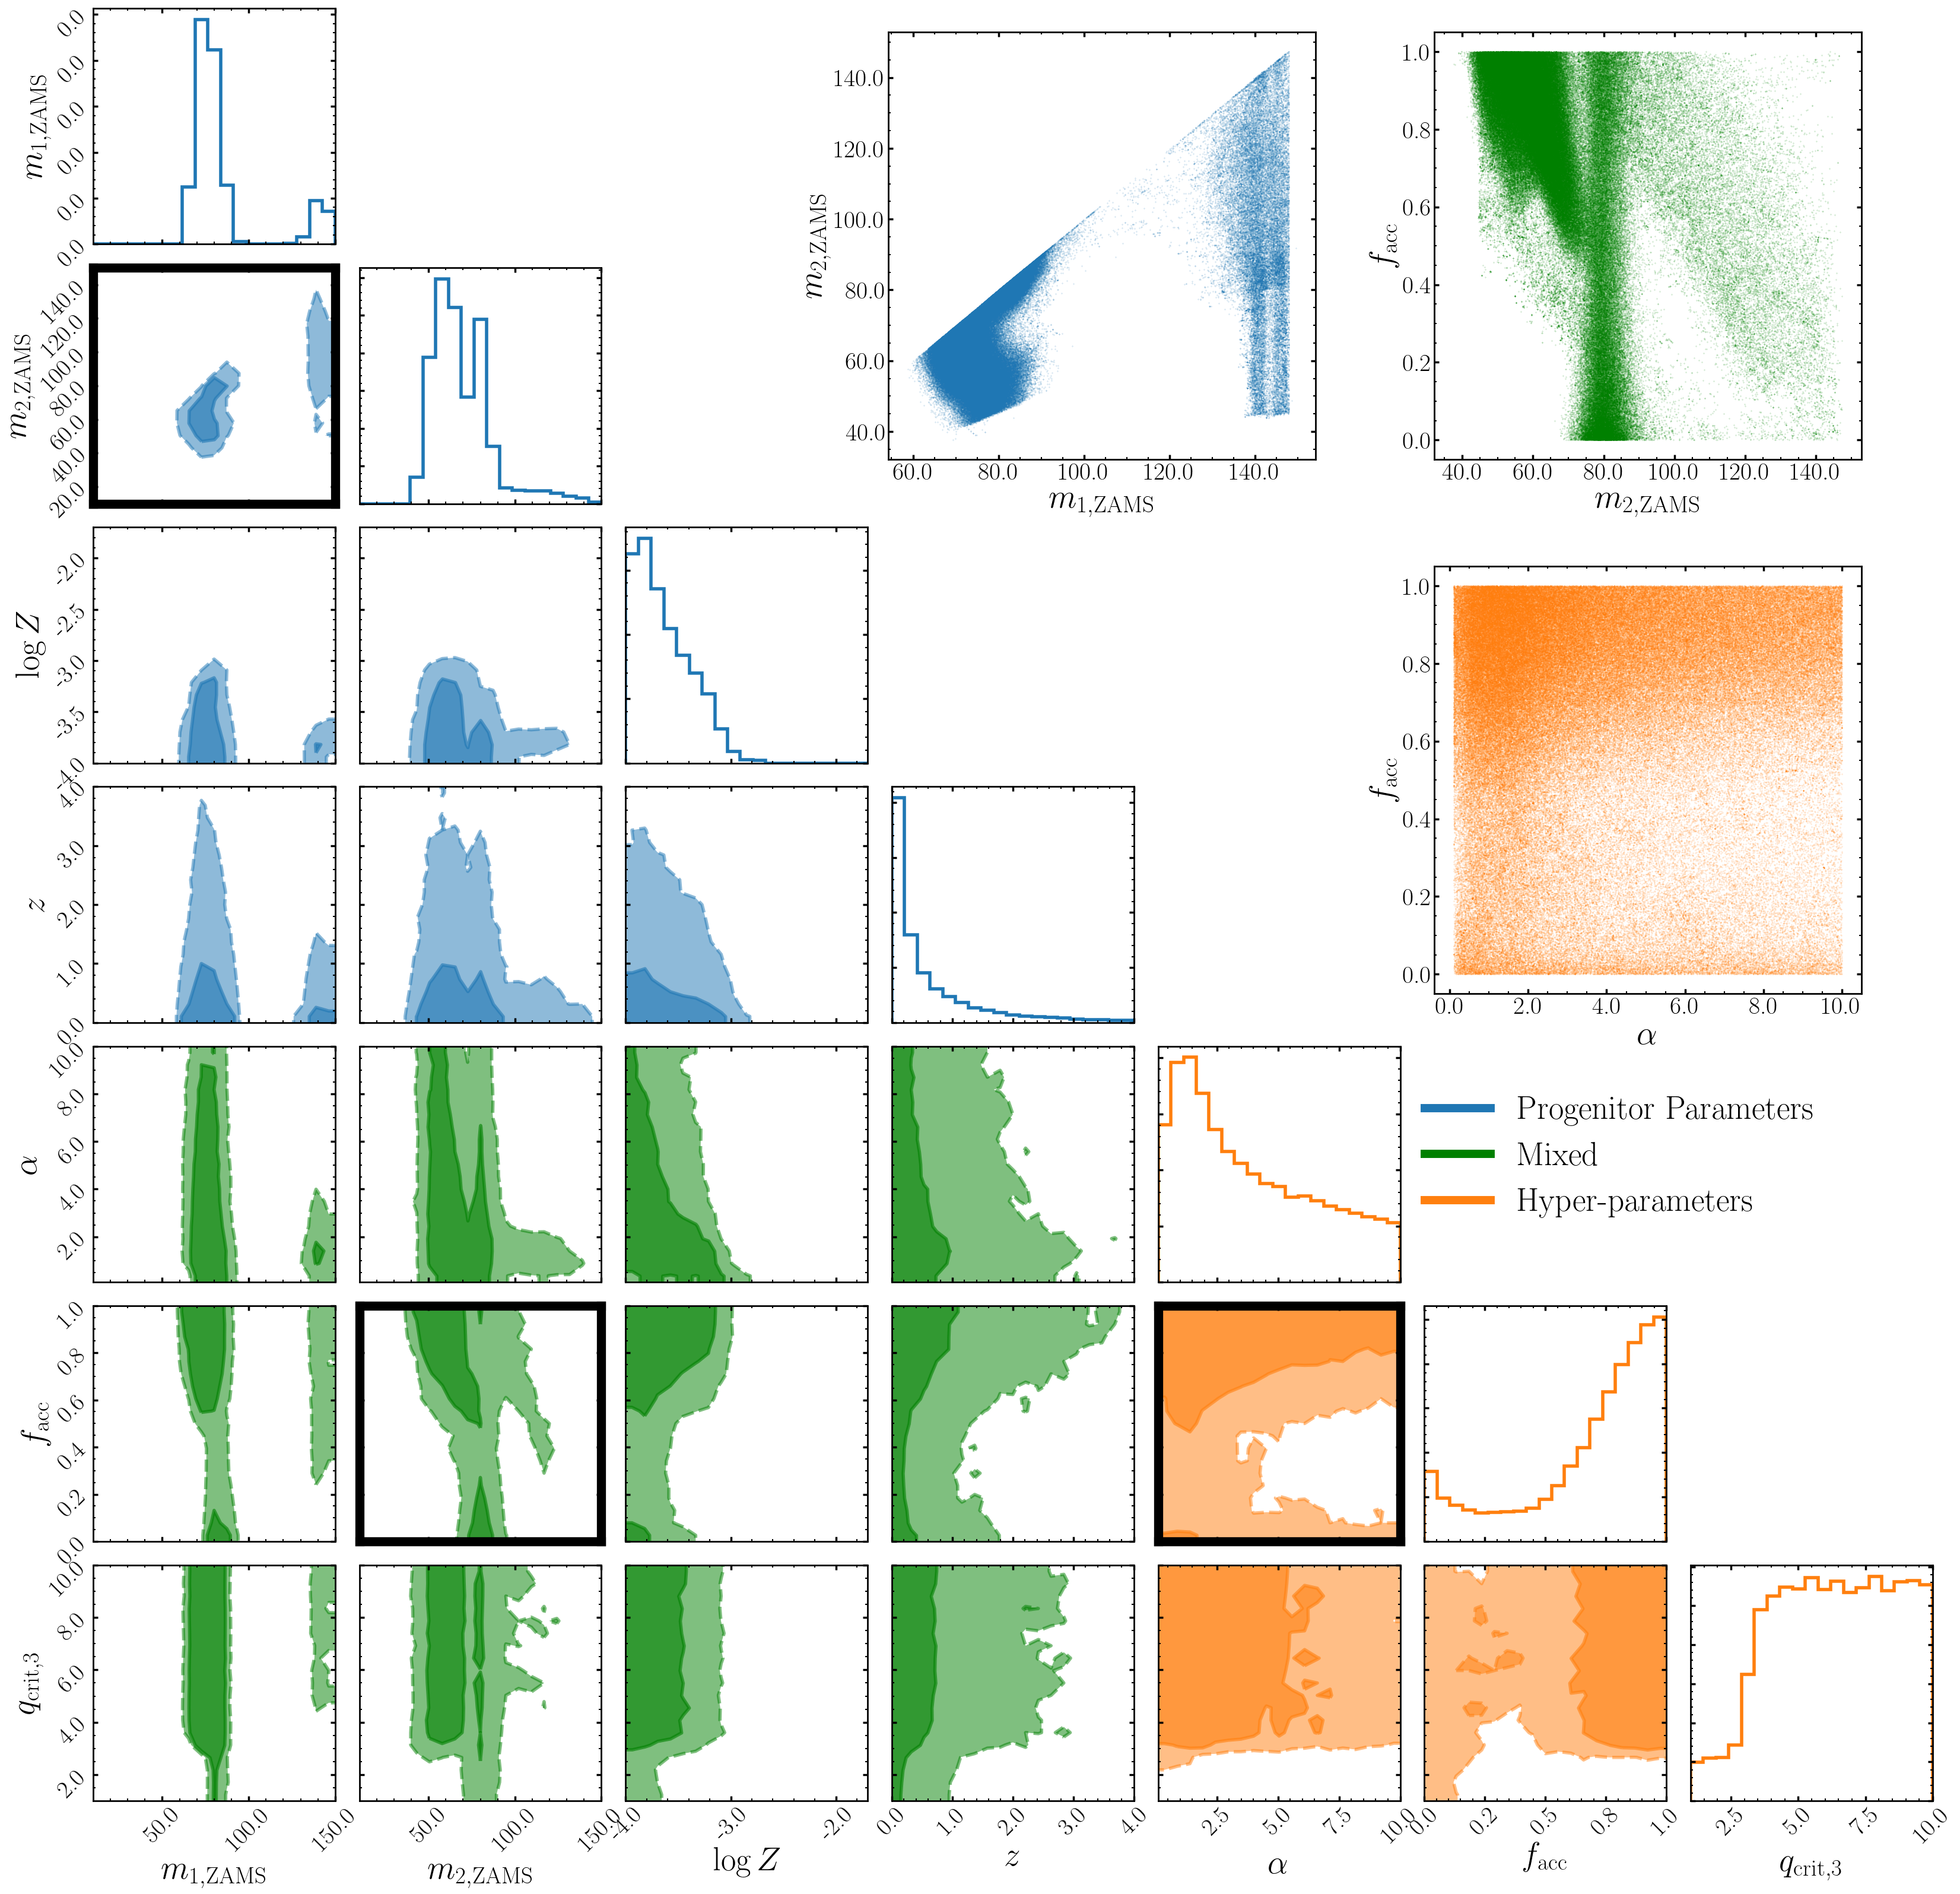
\includegraphics[width=\textwidth]{static/GW150914_corner_zoomed_lowres.png}
    \caption{The posterior for GW150914 in both the progenitor parameter space and hyper-parameter space.
    $M_1$ and $M_2$ are the progenitors' masses. $\log{Z}$ is log metallicity at ZAMS.
    $z$ is the redshift at ZAMS. 
    $\alpha$ is the common envelope efficiency.
    $f_{\rm acc}$ is the fraction of mass accreted during stable mass transfer.
    $q_{\rm crit 3}$ is the critical mass ratio on the Hertzsprung Gap,
    Note that the redshift is not fitted during the root finding process or the MCMC process.
    Once we have find the evolutionary parameters, we add the delay time to the lookback time of the observed posterior sample,
    then from the total lookback time we can compute the redshift at ZAMS.
    We highlight three panels in the corner plots to show the fine structure of the set of posterior samples in the evolutionary parameter space.
    We also color the posterior in a particular panel according to the type of parameters involved in the corner.
    Blue denotes panels that include only progenitor parameters,
    green denotes panels that include a mix of progenitor and hyperparameters,
    and orange denotes panels that include only hyperparameters.
    }
    \label{fig:GW150914_posterior}
\end{figure*}

% \kw{Talk about implication on single event posterior.}
Once we obtain a set of binaries which successfully map the ZAMS parameters and hyperparameters to BBH merger masses, 
we re-evolve the set of ZAMS parameters with the same physical assumptions as A21, but vary the common envelope efficiency 
to explore how keeping a fixed model which only varies one hyper-parameter affects our analysis. 
Figure~\ref{fig:compare_fixed_variable} shows the distribution of ZAMS masses for three models (first through third columns), 
each with a different $\alpha$ but the same hyperparameters as A21, 
as well as the results of our sampling which allows our hyperparameters to vary (fourth column). We find that holding the accretion 
efficiency, common envelope and natal kick physics to fixed values greatly reduces the ZAMS parameter space 
that produces GW150914-like mergers. In contrast, by allowing the hyperparameters to fully span the model uncertainty, we 
find that there are distinct ZAMS parameters which produce GW150914-like mergers and conversely, ZAMS parameters which 
fail to produce GW150914-like mergers \emph{regardless of our hyper-parameter choice.}
\kw{@Katie, can you put a frame around the fourth column highlighting it is this work?}



\begin{figure*}
    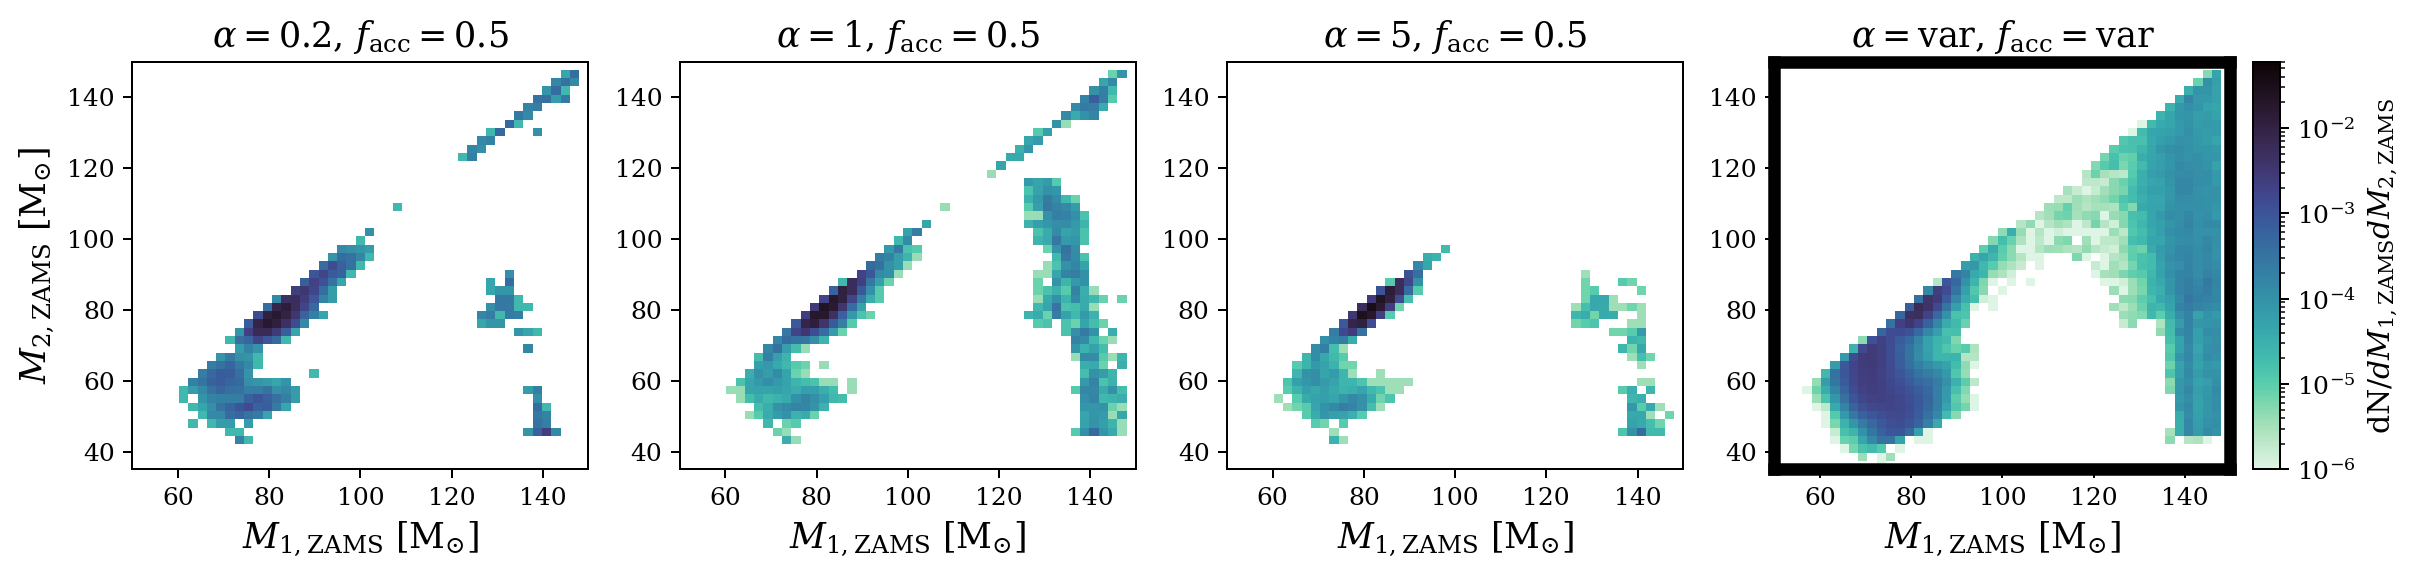
\includegraphics[width=0.98\textwidth]{static/compare_fixed_variable.png}
    \caption{Comparison of ZAMS masses for binaries which produce GW150914-like mergers for three variations of $\alpha$
     with fixed set of parameter assumptions matching those of A22 (first three columns) and for binaries which produce 
     GW150914-like mergers when $\alpha$, $f_{\mathrm{acc}}$, and $q_{c,3}$ are allowed to vary, (fourth column).}
    \label{fig:compare_fixed_variable}
\end{figure*}

% Validity paragraph
To check the validity of the recovered posterior, it is essential to check whether it is consistent with the original posterior in the observable space.
We reproject the recovered posterior to the observable space, and compare the KL divergence between the original posterior and the reprojected posterior.
In particular, we compute KL divergence of the samples obtained from root-finding alone and after MCMC sampling.
For GW150914, the KL divergence between the reprojected posterior and the original posterior is \kw{fill later} nats on average if we use the root-finding result alone,
whereas the MCMC result has a higher KL divergence at \kw{fill} nats.
The KL divergence stays stable for reprojecting with different random seeds. 
\kb{Can we show this in the figure somehow? Maybe like KL divergence as a function of reprojection number as a lower small panel?}
\kw{The problem with that is it is basically one dot or a flat line, which is very unentertaining. I wouldn't necessarily want to make a figure out of the KL divergence just because it is pretty boring and distracting.}
In fig.\ref{fig:GW150914_reprojection}, we can see the reprojected posterior from both the root-finding process alone and the MCMC result agrees well with the original posterior,
even though the agreement between the MCMC result and the original posterior is not perfect. 
This degradation of the agreement comes from the fact that we are using a KDE to estimate the posterior density in the observable space.
Note that the result from root-finding alone and the result from MCMC agrees well in the evolutionary parameter space.
Compared to the result shown in a previous study, our result covers almost all the posterior of GW150914 in the masses space,
which means our result is more consistent with the observation.


\begin{figure}
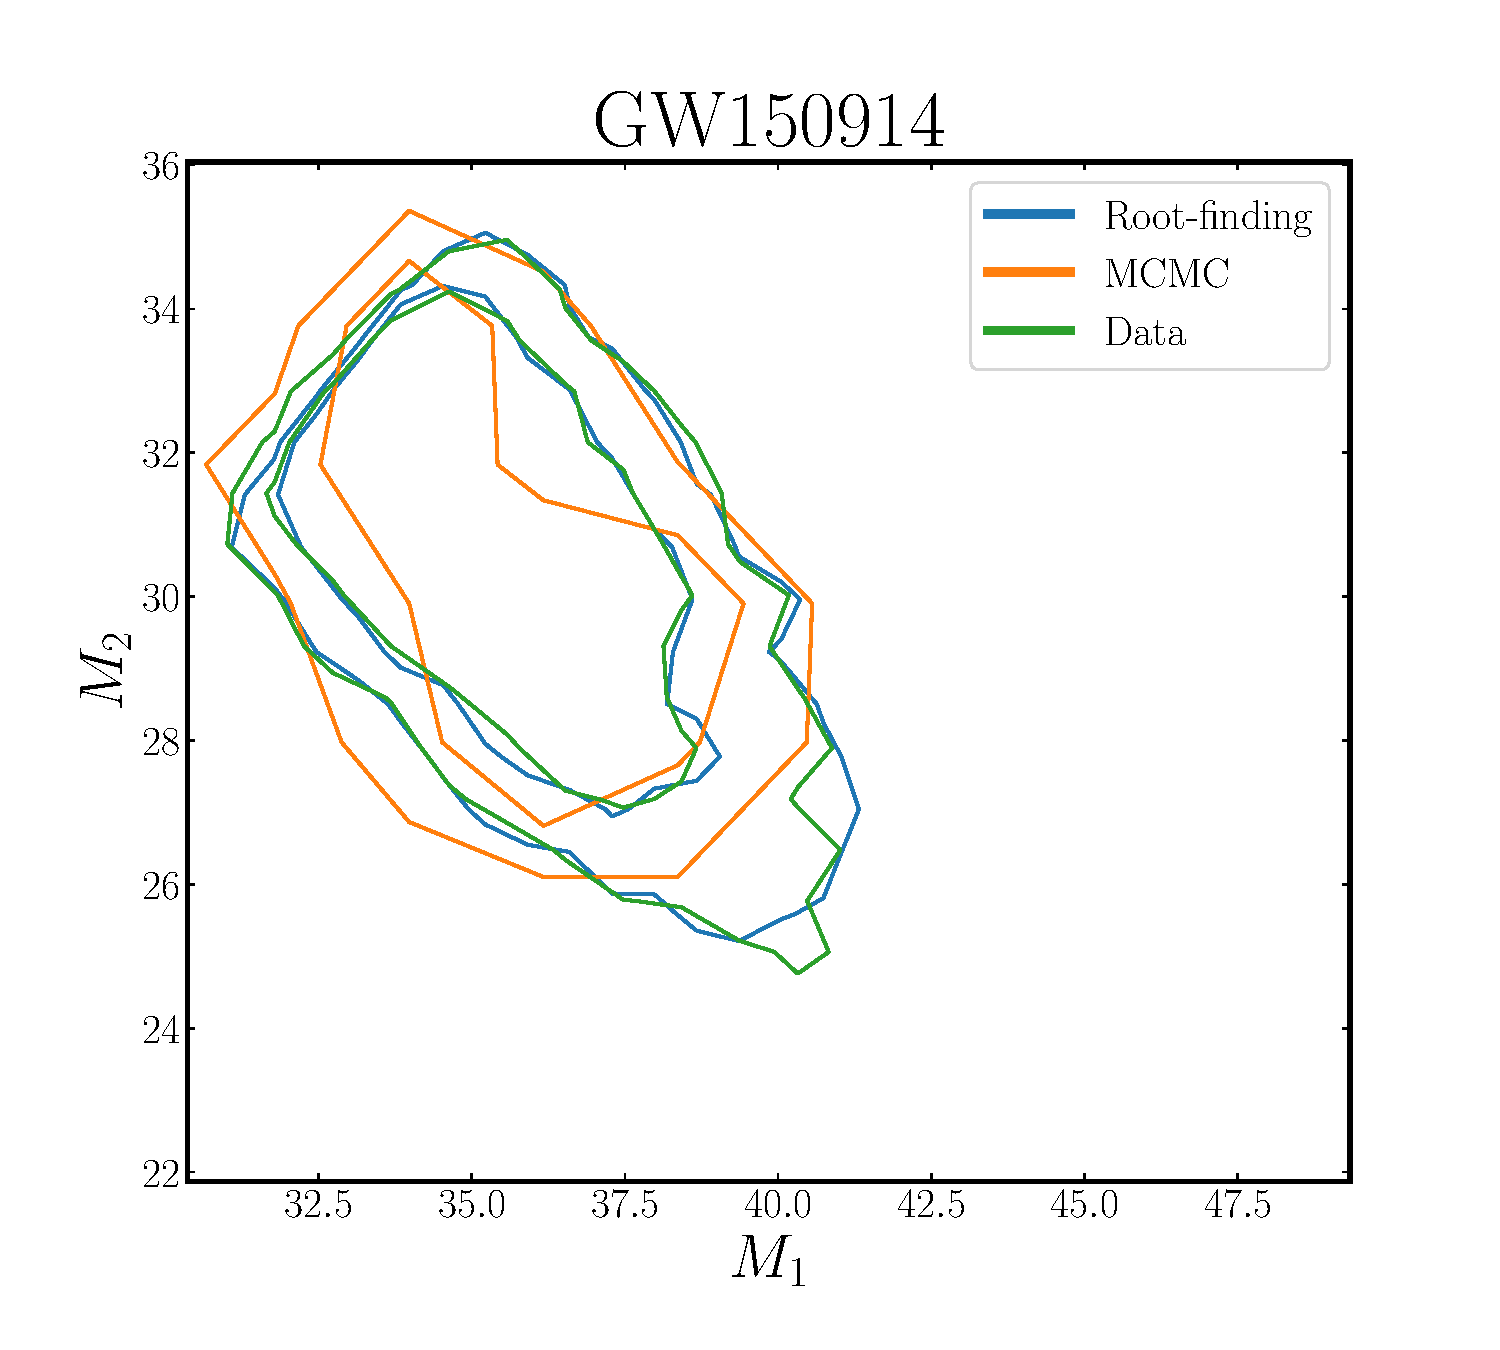
\includegraphics[width=0.49\textwidth]{static/GW150914_reprojection.pdf}
\caption{Reprojecting the posterior in evolutionary parameter space of GW150914 to observable space.
The blue contour is the reprojected posterior after the root-finding procedure.
The orange contour is the reprojected posterior after the MCMC procedure.
The green contour is the posterior plotted using the original LVK posterior samples.
}
\label{fig:GW150914_reprojection}
\end{figure}


% Paragraph discussing the potential application on the population side.
To illustrate the potential benefit of our method on the population level, we perform the same analysis for all events in GWTC3.
Plotted in figure \ref{fig:GWTC3_f_acc_mass} is the posterior density in the $m_{1,{\rm GW}}-f_{\rm acc}$ space for most of the events in GWTC3.
Each contour represents the $68\%$ credible interval of the posterior density for that particular event.
Although it does not conclusively suggest a dependency between $f_{\rm acc}$ and $m_{1,{\rm GW}}$,
there is a suggestive trend showing $f_{\rm acc}$ could possibly increase as the mass of the progenitor increases.
This means the stable mass transfer (SMT) phase of a light binary is preferably non-conservative, whereas the heavier the events are, the more likely their SMT is conservative.

Note that some events did not pass the KL divergence test we proposed in section \ref{sec:method}, which we do not include in figure \ref{fig:GWTC3_f_acc_mass}.
Low mass events are more subjected to random fluctuation because natal kick is less modulated by fallback in lighter system,
which can lead to a final system either with or without a merger event randomly,
so the reprojected posterior may not agree with the original posterior in the observable space consistently, hence yielding a higher KL divergence on average.
On the other hand, \texttt{COSMIC} struggles to produce events above the pair instability supernova mass cutoff $m_{1,{\rm GW}}$,
so the posterior in the evolutionary parameter space only correspond part of the posterior in the observable space, therefore events beyond the PISN mass gap has higher KL divergence.
Events with more extreme mass ratios are not likely to be recovered by the method. \kw{@Katie gives reason?}

The point of figure \ref{fig:GWTC3_f_acc_mass} is to show this method could in principal reveal the correlation between progenitor parameters and hyperparameters on a population level.
A careful treatment of all event in the catalog and discussion related the physical implication of figure \ref{fig:GWTC3_f_acc_mass} is beyond the scope of this paper,
therefore we defer a detail study of the physics related to the population of GW events in the future.
Also, despite some events do not pass the KL divergence test, we can still see the correlation in the region where the events are neither affected by randomness nor the PISN mass gap.


\begin{figure}
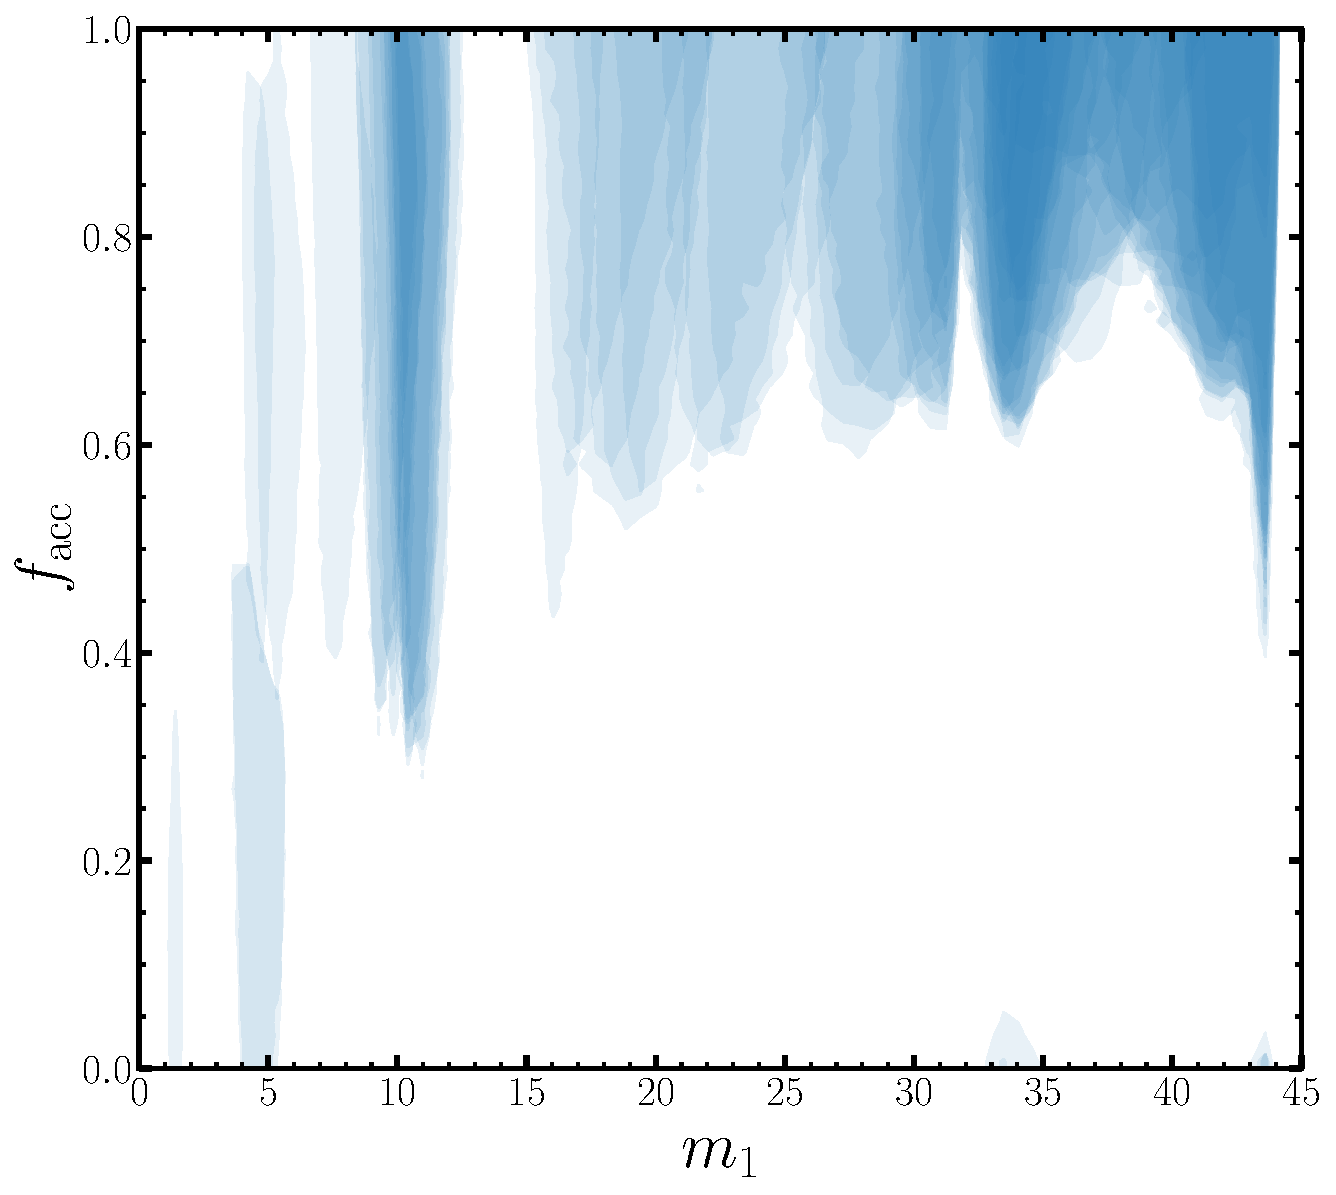
\includegraphics[width=0.49\textwidth]{static/GWTC3_f_acc_mass.pdf}
\caption{
    The posterior density in the $m_{1,{\rm GW}}-f_{\rm acc}$ space for most of the events in GWTC3.
    Each contour is the $68\%$ credible interval of the posterior density for a particular event. \kw{Check interval number}
    At $m_{1,{\rm GW}} \sim 45 M_{\odot}$, the pair instability supernova mechanism prevents \texttt{COSMIC} from producing events that are more massive than this cutoff.
    Therefore, events with the majority of posterior support above this cutoff is not compatible with \texttt{COSMIC}, hence has a large KL divergence and excluded from this figure.
    On the low mass end, neutron star binaries or neutron star-black hole binaries are subjected to randomness induced by the natal kick,
    also resulting in a larger and fluctuating KL divergence, therefore they are also excluded from the analysis.
}
\label{fig:GWTC3_f_acc_mass}
\end{figure}

\section{Discussion}
\label{sec:discussion}


We present a new pathway to understand binary evolution with GW events in this paper.
Instead of forward modelling an assumed distribution of initial binary to the observed population,
we find the corresponding evolutionary parameters for each GW events. 
In this work we first showcase the power of the proposed method with GW150914.
We show the joint posterior of the two events' progenitor parameters and hyperparameters.
In particular, to the authors' knowledge, this is the first time the correlation between progenitor parameters and hyperparameters is explored.
Our work is not only a more efficient way to study GW events' progenitors,
but also allows the possibility of measuring the astrophysics related the binary evolution, especially in capturing the correlation between different hyperparameters.

To further illustrate the power of the method, we show the inferred fraction of accretion during SMT depends on the progenitor masses.
The most obvious advantage our method provides is it returns the joint posterior distribution of progenitor parameters and hyperparameters for each event.
This enables a data-driven way to study the distribution of hyperparameters,
i.e. once we have a catalog of events, each has their own set of posterior in the hyper-parameter space,
we can employ common techniques such as hierarchical Bayesian analysis to fit a population model to the distribution of hyperparameters,
without making specific assumptions such as fixing the hyperparameters for all types of event.

% Rate analysis is now just counting, like what's done in phenomenological model, instead of forward modelling.
Another perk of our method is the "rate" calculation is now independent of
assumed initial condition such as a particular star formation rate model, which
is a dominant factor of uncertainty for rate prediction in the past. Once we
have pull back the GW event posterior from the observable space to the
evolutionary parameter space, we can apply the same methods we use to account
for the rate in the observable space. In the observable space, the overall rate
is basically a normalization that is defined in the local universe i.e. the
local merger rate. \kw{cite} In the evolutionary parameter space, we can instead
fit for the production rate of merger events at some redshift. This also means
one can study the progenitor-formation rate in a data-driven manner instead of
assuming a particular model. \wf{Emphasize this more---build up the SFR directly
from a population of GW events, with realistic assumptions about the dtd.}


% Single formation channel and fundamental limitation on that.
While our method allows data-driven exploration of the hyperparameters space for the first time, there are a number of improvements can be implemented in future studies.
In this study we use only \texttt{COSMIC} as our evolutionary function, which by design cannot explain all the events in GWTC3.
For example, event with either of the component mass larger than the PISN gap such as GW190521 cannot be explained by \texttt{COSMIC}.
Alternative channels such as dynamic formation channel will be needed to explain some subset of the events in GWTC3.
As pointed out in the literature \kw{Cite mike}, it is unlikely that all the observed events in GWTC3 can be explained by a single formation channel.
As GW detectors sensitivity increase, we expect to see more and more events that are unusual in some way.
Therefore, having a self-consistence population synthesis code that contains multiple formation channels is essential to accommodate the growing catalog of GW events.
In this paper, our main focus is to illustrate the concept of "back-propagating" GW events posterior sample in this work,
highlighting the capability of our method and motivating the community to build the next generation population synthesis code that can work with our method.
To avoid cluttering of focus, we discuss the physical implication of the result presented in this work under our specific assumption (i.e. using \texttt{COSMIC} as our evolutionary function) in a companion paper.


% Randomness paragraph
Due to the implicit definition of random variables in \texttt{COSMIC}, our evolutionary function is stochastic.
This introduces significant inefficiency in our root-finding and sampling algorithm.
The main stochasticity in \texttt{COSMIC} comes from natal kick, which significantly affect the evolution pathway of low mass events such as BNS events.
The effect of natal kick is suppressed for heavier mass events due to fallback.
This means events with lighter masses are subject to stochasticity of the function,
where the sampling process for heavier events behaves as if the evolutionary function we use are deterministic.
% Indeed, we see this behavior in a couple of case studies.
% For heavy event such as GW150914, the reprojected posterior agrees with the data posterior.
% For light event such as GW170817, although during the root-finding process the convergence criteria is met,
% the reprojected posterior does not agree with the data posterior.
Due to computational limitation, we only try 1000 different initial guesses per posterior sample in the root-finding process.
This means any posterior sample that has a probability of merging rarer than 1 in 1000 could be missed.
Obviously the problems which comes with the randomness can be alleviated by performing more tries per posterior sample,
but this is not scalable in practice.
On top of limitation in efficiency, some formation channels require explicit control of random variables by construction.
For example, in a dynamical formation scenario such as binaries that form in a globular cluster,
each binary has some probability of undergoing a multi-body encounter with another member in the cluster.
These encounter probability distributions are either studied with direct N-body simulations or semi-analytical methods.
In both cases, each member of the cluster is no longer completely independent of the other members, but coupled through the encounter probability distribution.
By studying the encounter probability distribution, we can infer the properties of the environment which the binary lives in.
This can only be done if we have explicit control over the random variables that characterize the encounter probability distribution.

% Need for selection bias to recover intrinsic distribution



% Gradient decending in the evolutionary parameter space is much more efficent than rejection sampling.
% Potential pitfall of interpreting this result.
% Need for full autodiff.

% By leveraging gradient-based optimization strategy, obtaining posterior samples in the evolutionary parameter space is much more efficient than rejection sampling.
% In each optimization step during the root-finding process, the current state of the guess and its gradient provide useful information about where the root might be.
% In contrast to sampling algorithm, which discard the sample whenever it is not accepted.
% This greatly benefit the efficiency of the root-finding process.
% On the other hand, this method is not a sampling algorithm, but a coordinate transform of the posterior samples.
% One should pay extra caution in interpreting the posterior samples in the evolutionary parameter space.
% Since posterior samples in the observable space can in principle have multiple roots in the evolutionary parameter space,
% the relatively weighting of these roots becomes ambiguous when the number of roots is large.
% For example, should we consider roots that are close to each other a single root or multiple roots?
% If we have two clusters of roots, the relative number of roots within each cluster would determine the relative weight of each mode.
% Note that since they both map to the same observable posterior sample within the acceptance threshold, all weighting assigned are equally valid from a "matching data" standpoint.
% This leave the interpretation of the posterior in the evolutionary parameter space ambiguous.
% In our case, we found empirically each posterior sample may at most only correspond to a handful of roots (most of the posterior samples have a unique root.), therefore we choose to assign equal weight to each root.

% The potential reason for the good agreement between MCMC and the root finding is due to the behavior of posterior in the evolutionary parameter space are larger determined by the posterior distribution in the observable space instead of multiple possible roots per posterior sample.
% We have also compared two MCMC results, one is initialized using the roots and another is initialized using samples drawn from a uniform prior.
% We found empirically the MCMC result using the roots as initialization converges at least an order of magnitude faster than the uniform prior initialization.
% This makes sense since the roots basically eliminate the long burn-in needed to go from random location in the evolutionary parameters to the most probable region.
% We leave a detail comparison between this method and direct sampling to future studies.

Another technical note is we use finite differencing to estimate the gradient of the objective function, which could be a significant source of error near transition points in the evolutionary parameter space.
Also, finite differencing is increasing inefficiency as we increase the dimensionality of the problem.
To improve the accuracy and efficiency in estimating the gradient of objective function, automatic differentiation is a promising feature that modeler should consider incorporating in their population synthesis code in the future.


To summarize, we propose a novel method to recover the posterior samples in the evolutionary parameter space for each GW event.
We point out hyperparameters in the usual population synthesis simulation context are not actually parameters related to the population,
but parameters about the evolutionary function.
This means the binary evolution functions can be constrained on an individual event basis.
We "back propagate" the posterior in the observable space to the evolutionary parameter space,
thus allowing us to study hyperparameters and its correlation with progenitor parameters in a data-driven manner.
Our method makes less assumption than the traditional forward modelling approach,
which often fix the hyperparameters across the entire population.
Since we are not limited to the fix hyperparameters assumption, we can explore the behavior of the hyperparameters across the population much more efficiently.
While our work lay down a data analysis pathway to understand the population of GW events,
no physics can be learned without a comprehensive physical model.
We hope this letter would motivate the community to build the next generation population synthesis codes that have the following properties:
first, they should have explicit control over the random variables so marginalizing over random variables can be done more precisely;
second, they should be as automatically differentiable as much as possible so exploring the evolutionary parameter space is efficient.
Combining this work and the next generation population synthesis code,
we can explore the full parameter space of binary evolution models with the next-generation GW detectors network in the near future.


\section{Acknowledgement}

\bibliography{bib}

\end{document}
